\section{Introduction}
\label{sec:introduction}

% state the learning objective 
The objective of this laboratory assignment is to choose the architecture of the envelope and voltage regulator circuits in order to have the best merit (M) possible. \par
Firstly, we started this laboratory writing an NGspice script that simulates the AC/DC converter and measure the output voltage level and voltage ripple , ploting the the voltages at the output of the envelope detector and voltage regulator circuits and the output AC component + DC deviation).\par
Then, using octave, we have created a theoretical model able to predict the output of the envelope detector and voltage regulator circuits, ploting the same results as in simulation analysis (using theoretical analysis). Finally, also the output DC level and the voltage ripple were computed. \par

The merit is calculated using the following expression:\par
\begin{equation}
    M = \frac{1}{Cost(ripple(v_0)+average(v_0-12)+10^{-6})}
\end{equation}\par
Where: \par
Cost = cost of resistors + cost of capacitors + cost of diodes \par
Cost of Resistors = 1 monetary unit per kOhm \par
Cost of capacitor = 1 monetary unit per $\mu$ F \par
Cost of diodes = 0.1Monetary units per diode \par
Firstly, we have created a simple circuit and then we were updating the circuit to improve the figure of merit. The final circuit obtainned is the one shown below in figure (Fig.\ref{fig:circuito}): \par

\begin{figure}[H]
\centering
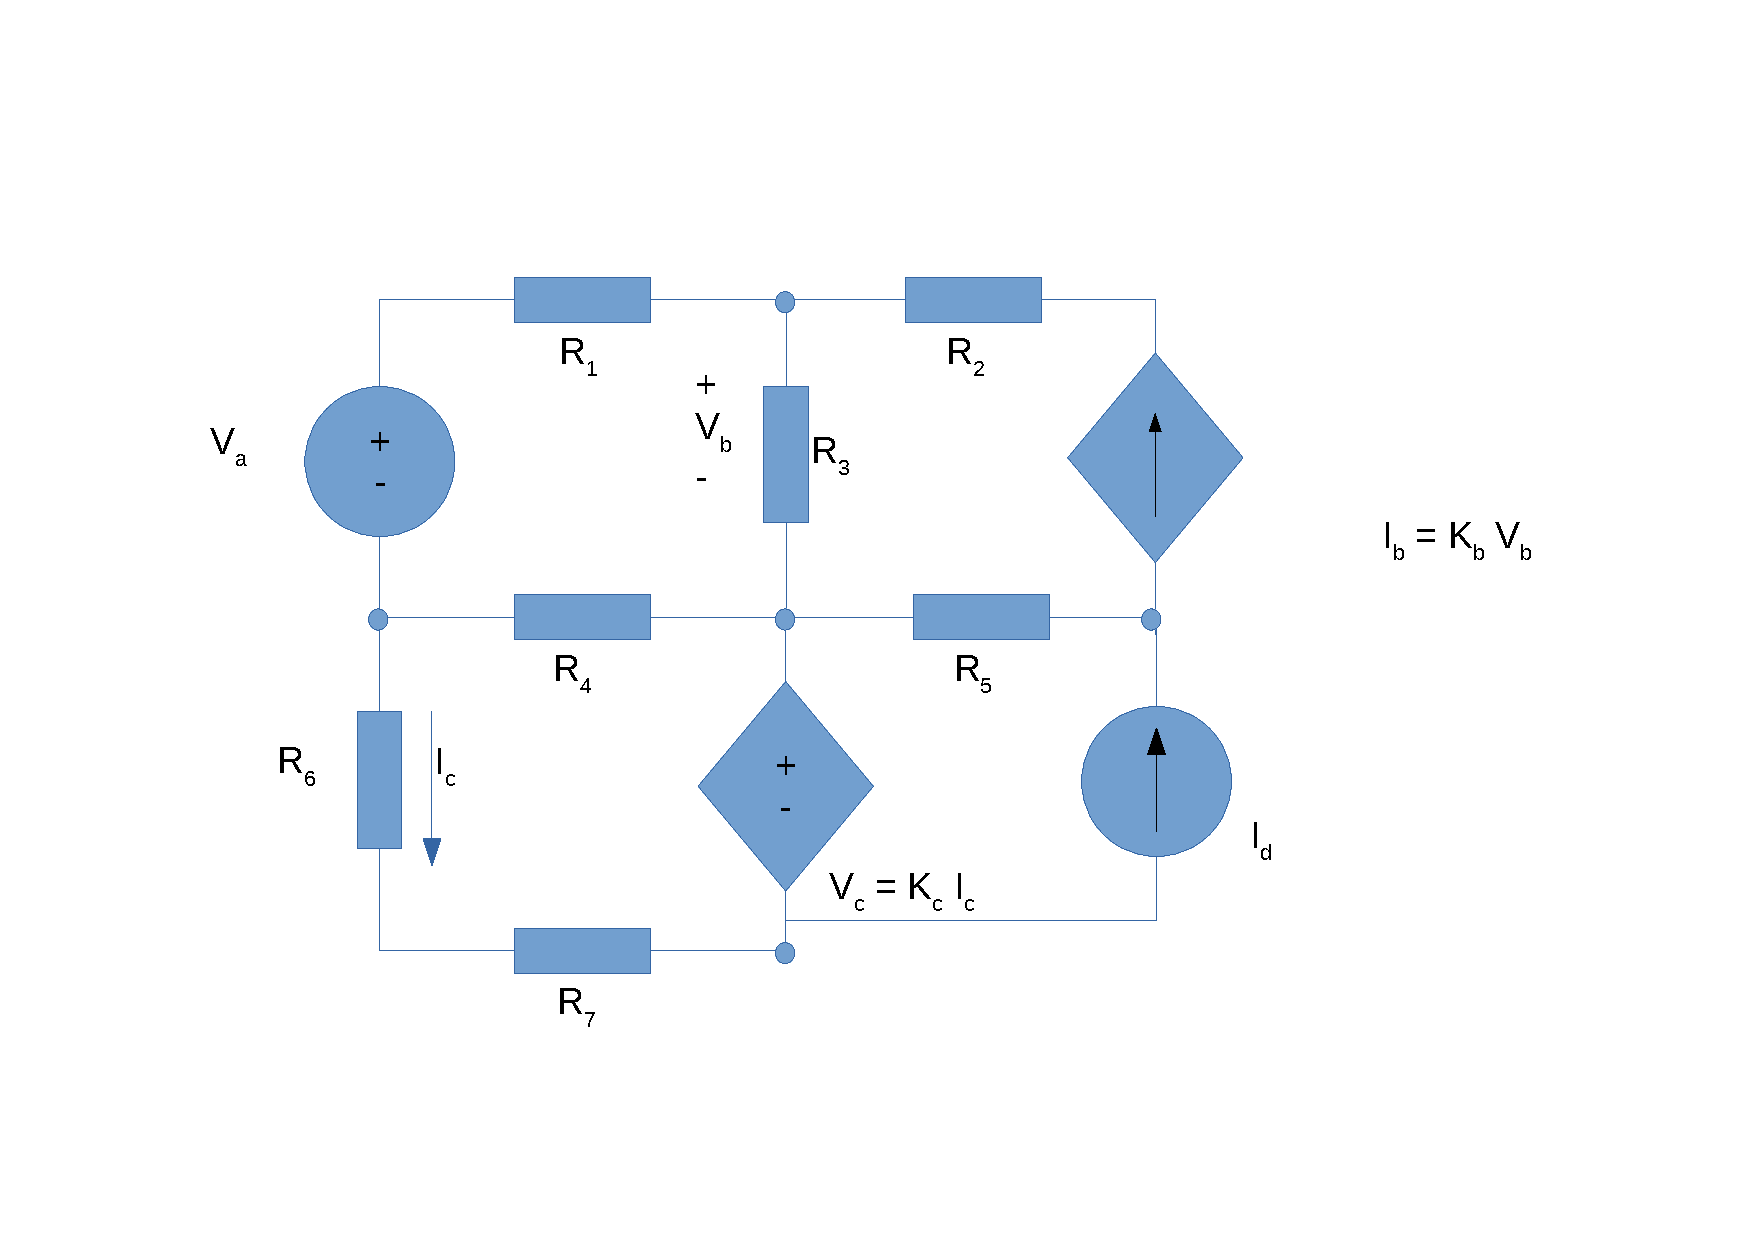
\includegraphics[scale=0.6]{circuito}
\caption{Final circuit}
\label{fig:circuito}
\end{figure}

The individual costs of the components used: \par
- Diodes - cost: 2.3MU; \par
- Capacitor - 5MU; \par
- Resistances - 55MU. \par

The data used was the following:

\begin{center}
  \begin{tabular}{ | c | c | }
    \hline    
    {\bf Name} & {\bf Value} \\ \hline
    $R$ & 27.3 k$\Omega$ \\ \hline 
    $C$ & 21 $\mu$S \\ \hline
    Diodes & 25 Units \\ 
    \hline
  \end{tabular}
\end{center}



